\section{Хэрэгжүүлэх PCG-н шийдэл}
Энэхүү бичвэрийн хүрээнд Dungeon-Crawler тоглоомын орчин үүсгэнэ. Системийн нэр "ControllerLevelGenerator" ба энэ нь Unity-н component.
\subsection{Dungeon-Crawler төрлийн тоглоом}
Энэхүү төрлийн тоглоом нь газар доор эсвэл олон өрөө тасалгаатай орчинд тоглогчийг олон янзаар(ихэвчлэн мангасуудын эсрэг тулалдах, аливаа оньсого тайлах, дүрээ сайжруулах зэрэг) сорьдог тоглоомын төрөл.  Тоглоомын орчин нь хязгаарлагдмал, тоглогчийн хийх үйлдэлд нөлөөлдөг тул тоглоомын орчин нь тоглоомын явцад нөлөөлөх байдал нь өндөр. Ийм төрлийн тоглоомд PCG-г ашигласан олон жишээ бий(Rogue 1985, Spelunky 2008, The Binding of the Isaac 2014).

\section{Системийн функциональ шаардлага}
\begin{itemize}
	\item Хэрэглэгч - ControllerLevelGenerator болон CellBundle-н тохиргоог хийх, шинээр CellBundle үүсгэх, шинээр CellUnit үүсгэх мөн эдгээрийг өөрчлөх.
\end{itemize}

\section{Функциональ бус PCG шийдлийн шаардлага}
\begin{itemize}
	\item Хурд

	      Орчныг нэг удаа тоглолт эхлэхэд үүсгэнэ. 2 секундийн дотор үүсгэнэ.
	\item Найдвартай байдал

	      Өрөө хоорондын хаалганы байршил нь зөв нэг өрөөнөөс аль ч бусад өрөө рүү дамжин явах боломжтой.
	\item Удирдах чадвар

	      Өрөөний үзэмж, орчны элементүүдийн тодорхойлох болон элементийн сонгогдох боломжийг удирдах боломжтой.
	\item Илэрхийлэлт болон олон талт байдал

	      Өөр хэмжээтэй өрөөнүүд, өрөөний элементүүд нь олон сонголттой байх.
	\item Бүтээлч байдал болон итгэж болох байдал

	      Өрөө нь хэт том эсвэл хэт жижиг биш. Хаалга болон шатны байршил нь тоглогч итгэж болох байх.
\end{itemize}

\section{Хэрэгжүүлэлт }
\section{Системийн class diagram}
\begin{itemize}
	\item Rectangle - Хоёр хэмжээст тэгш өнцөгтийг илэрхийлнэ.
	\item GridXZ - Гурав хэмжээсд ашиглах хоёр хэмжээст торон систем.
	\item GridCell - GridXZ-н нэгж
	\item CellBundle - Дотроо нэг сэдэвтэй CellUnit-үүдийн багц.
	\item CellUnit - Тухайн төрлөө илтгэх модель болон component-тэй prefab.
	      \begin{itemize}
		      \item Floor, Solid, Pillar, StairDown, StairUp, Abyss, Door, Empty гэсэн төрлүүдтэй.
		      \item 5м\textsuperscript*{2} харьцах хэмжээтэй орчны нэг нэгж.
	      \end{itemize}

	\item ControllerLevelGenerator - Тоглоомын орчныг үүсгэх хэрэглэгчтэй харилцах component, харилцах систем.
	      \begin{itemize}
		      \item Санамсаргүй тооцооллын Seed авдаг ба уг утгаар системийн орчны үр дүнг дахин боловсруулж болно.
		      \item Scene эхлэх үед тоглоомын орчныг үүсэх үйл явцыг эхлүүлэн системийг гол удирдах, хянах үүргийг гүйцэтгэдэг хэсэг.
	      \end{itemize}
\end{itemize}
\begin{figure}[H]
	\centering
	\caption{Class Diagramm}
	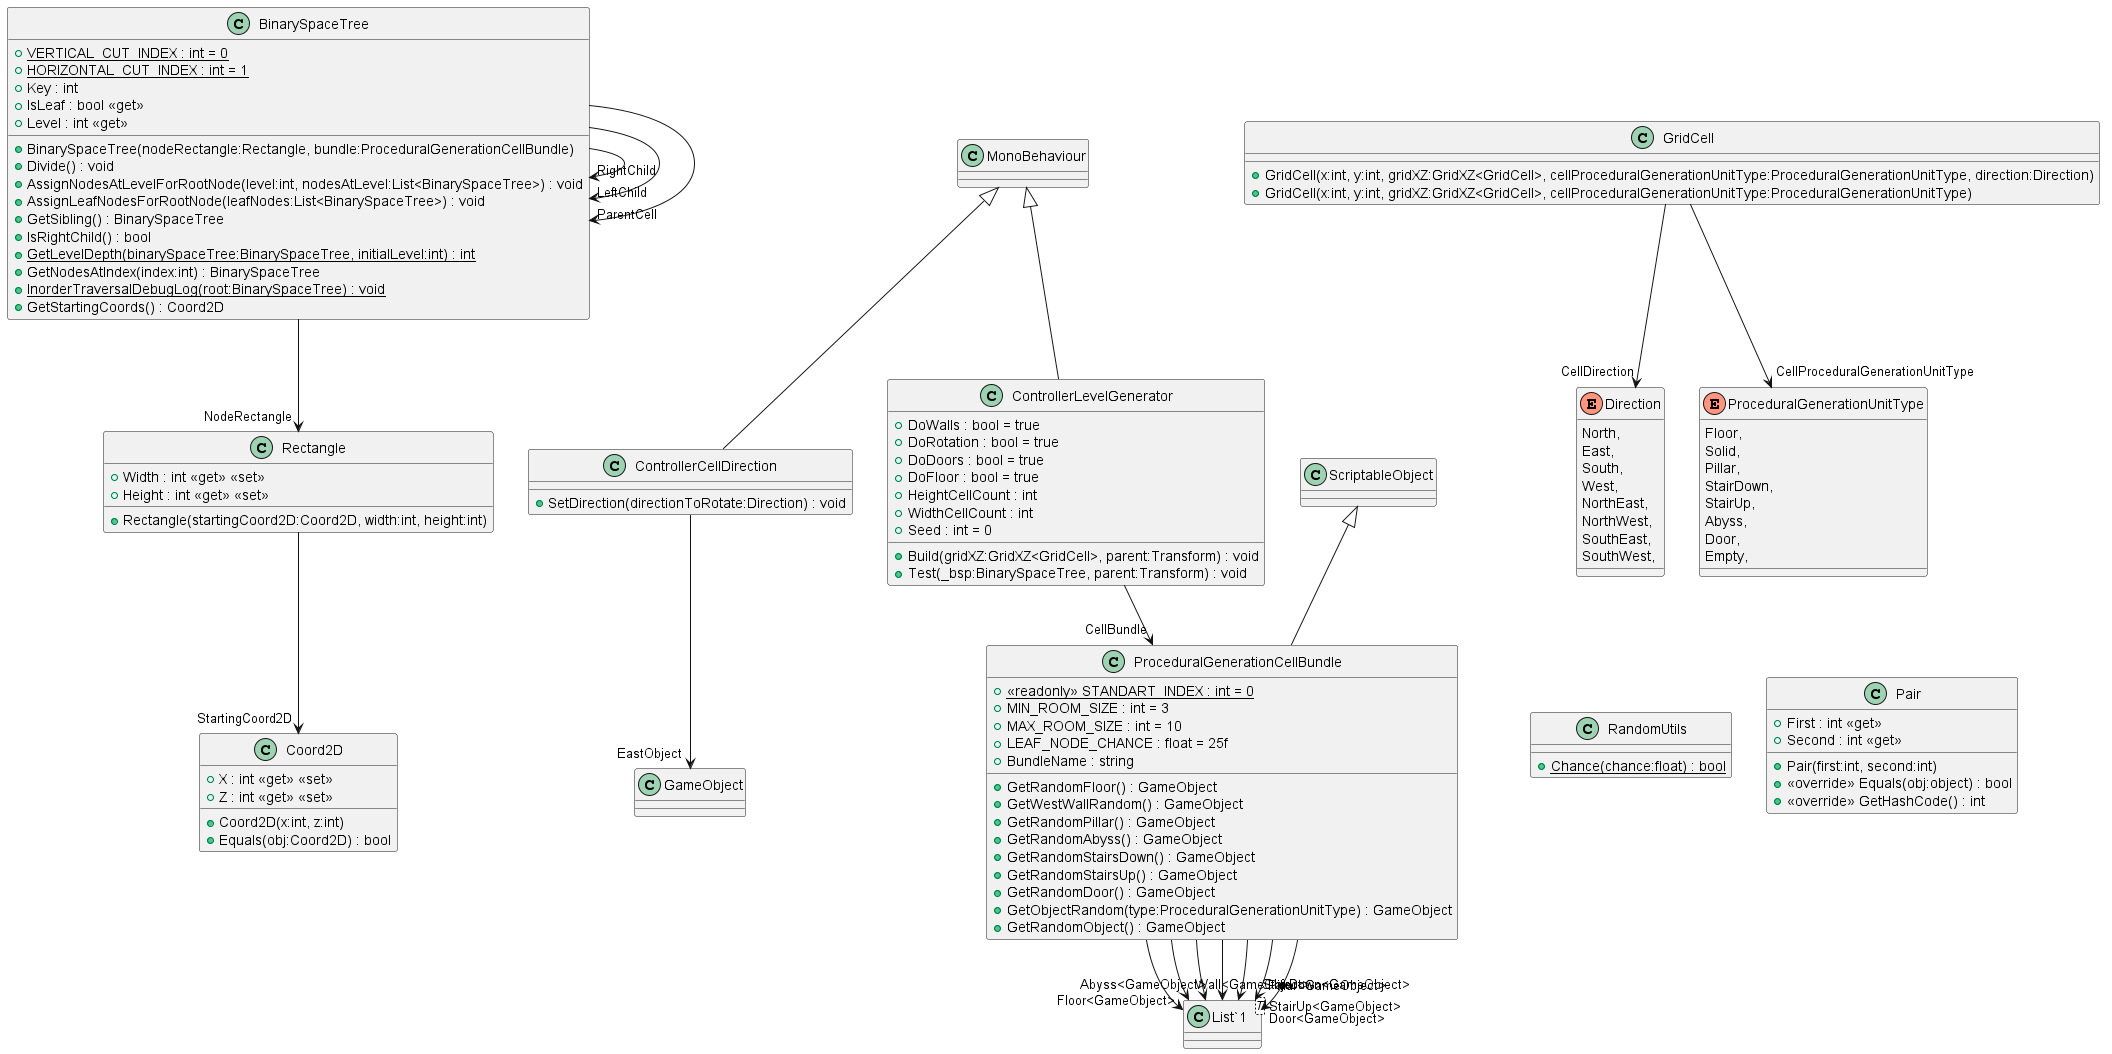
\includegraphics[angle=90, height=\textheight-1cm]{./images/ClassDiagramm.png}
	\label{fig:ClassDiagramm}
\end{figure}

\section{Хэрэглэгчийн харилцах хэсэг}

\subsection{CellBundle}

\begin{figure}[ht]
	\centering
	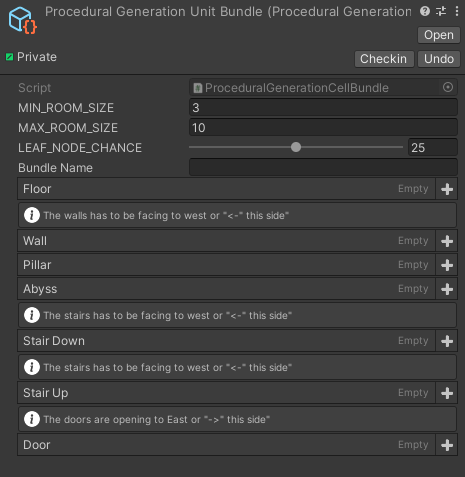
\includegraphics[width=\textwidth/2]{./images/user_interface_cell_bundle.png}
	\caption{Хэрэглэгчийн харилцах хэсэг - CellBundle}
	\label{fig:UserInterfaceCellBundle}
\end{figure}


\subsection{ControllerLevelGenerator}

\begin{figure}[hb]
	\centering
	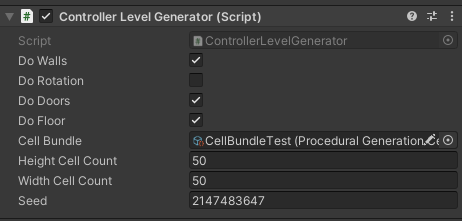
\includegraphics[width=\textwidth/2]{./images/user_interface_controller_level_generator.png}
	\caption{Хэрэглэгчийн харилцах хэсэг - ControllerLevelGenerator}
	\label{fig:UserInterfaceControllerLevelGenerator}
\end{figure}

\section{Системийн үйл явц}
Dungeon-crawler төрлийн тоглоомны орчныг процедурт шийдлээр үүсгэхэд ерөнхийдөө дараах гурван зүйлсийг хийдэг ба дараах байдлаар гүйцэтгэв.
\begin{itemize}
	\item Төлөөллийн загвар. Орчны өрөө тасалгааны ерөнхий бүтцийн энгийн загвар.
	      \begin{itemize}
		      \item Үүнийг хоёр хэмжээст торон системээр хэрэгжүүлнэ.
		      \item Торон системийн нэгж нь GridCell
	      \end{itemize}
	\item Төлөөллийн загварыг үүсгэх үйл явц буюу арга.
	      \begin{itemize}
		      \item Орчны ерөнхий бүтцийг BSP ашиглаж гаргана. Үүнд өрөөнүүдийн хэмжээ болон байршил нь торон системдээр тодорхойлогдоно.
		      \item Орчны ерөнхий бүтэц дээр нэмэлт өөрчлөлт хийнэ. Үүнд Floor, Door, Wall CellUnit үүдийг торон системд олгоно.
	      \end{itemize}
	\item Төлөөллийн загварыг бодит тоглоомын модел болгох үйл явц буюу арга.
	      \begin{itemize}
		      \item ControllerLevelGenerator нь GridXZ-н GridCell болгон дээр төрөл болон байршлын мэдээлэл дээр тулгуурлан CellBundle-с prefab-г Scene дээр үүсгэнэ.
	      \end{itemize}
\end{itemize}

\begin{figure}[t]
	\centering
	\caption{Sequence Diagramm эхний хэсэг}
	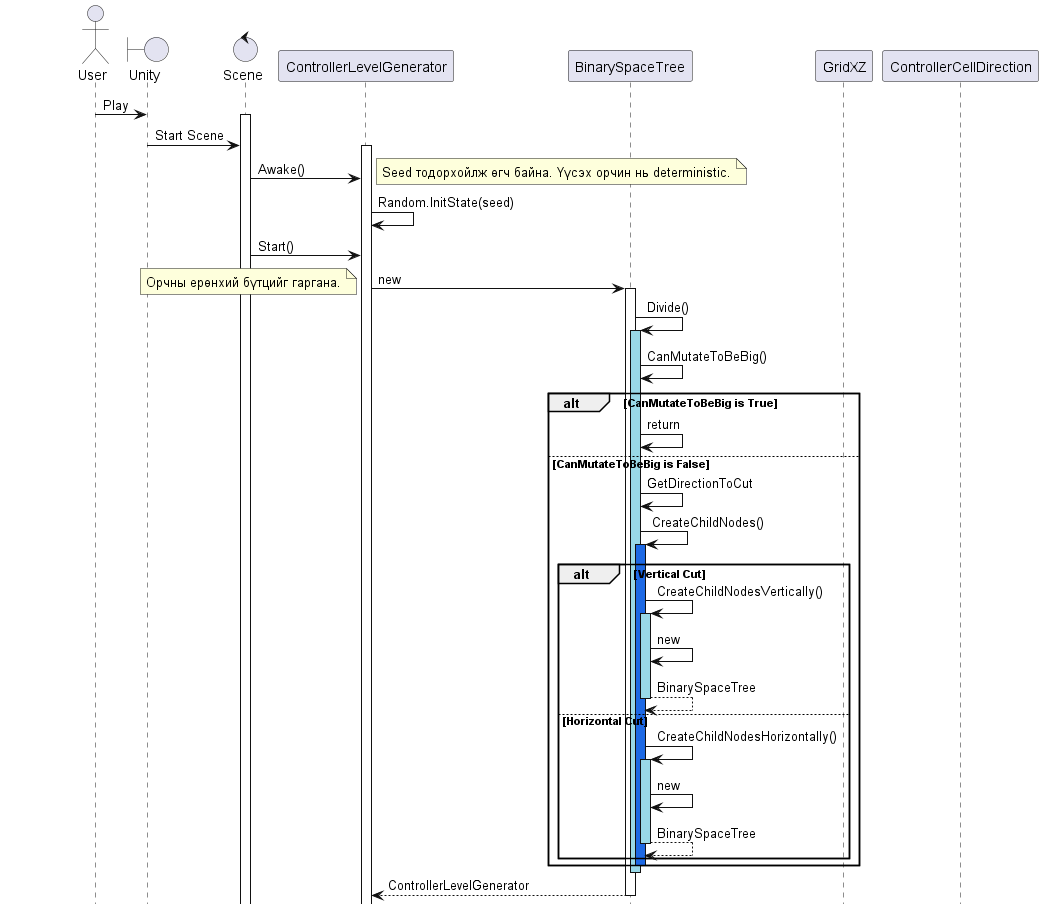
\includegraphics[width=\textwidth]{./images/sequence_1.png}
	\label{fig:SequenceDiagramm1}
\end{figure}
\begin{figure}[b]
	\centering
	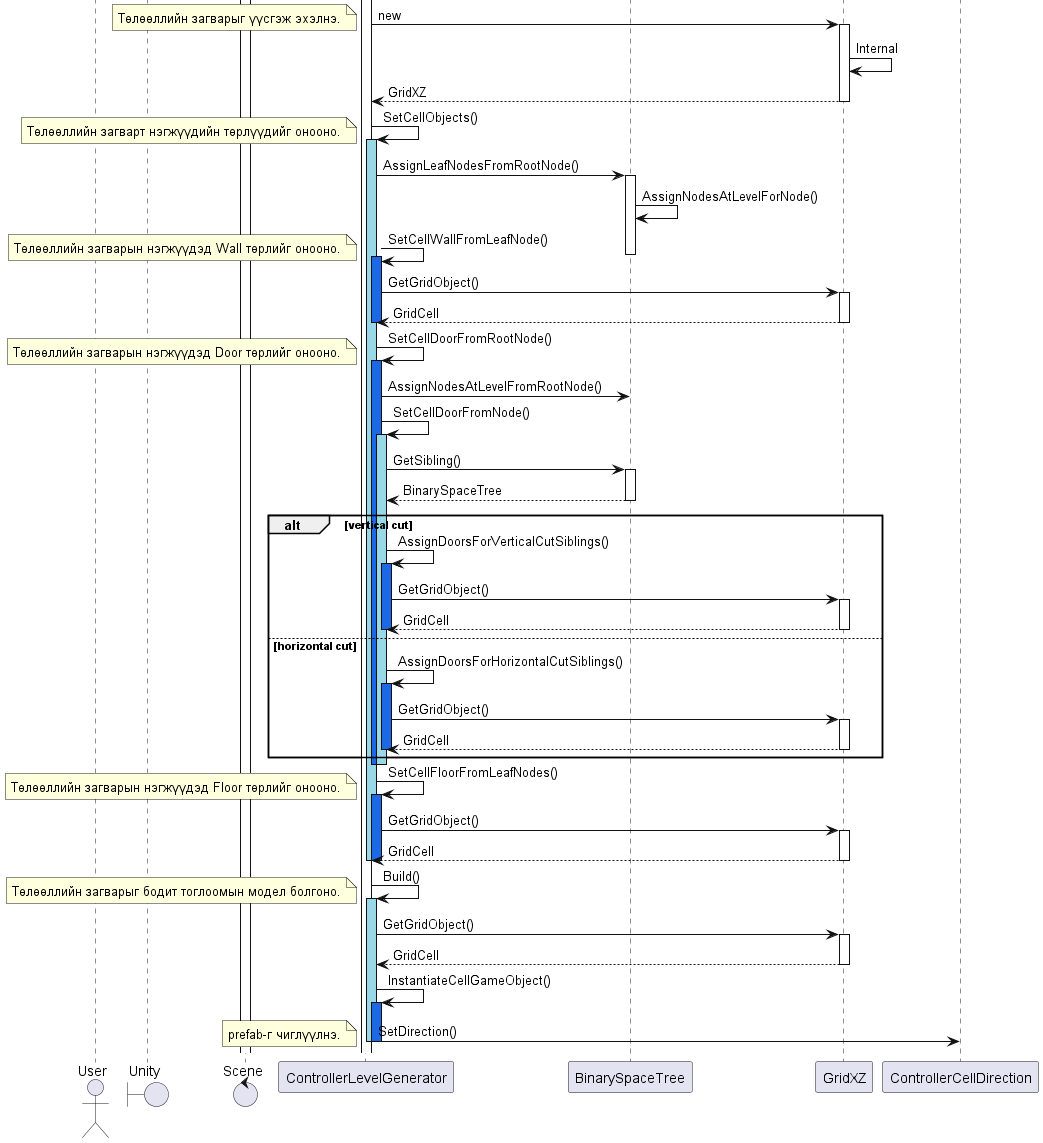
\includegraphics[width=\textwidth]{./images/sequence_2.png}
	\caption{Sequence Diagramm хоёр дахь хэсэг}
	\label{fig:SequenceDiagramm2}
\end{figure}


